\documentclass[
	11pt, % 10pt - 12pt
	%letterpaper
	%indonesian
]{assignment}

% Template-specific packages
\usepackage{mathpazo} % Use the Palatino font

\usepackage{graphicx} % Required for including images
\usepackage{booktabs} % Required for better horizontal rules in tables

\usepackage{amsmath} % Math!
\usepackage{amssymb} % Math symbols!
\usepackage{listings} % Required for insertion of code
\usepackage{enumerate} % To modify the enumerate environment

\newcommand{\ipAddress}[1]{{\fontfamily{cmtt}\selectfont #1}} % IP Address custom style!

% ! CUSTOM - LST Preset
\lstset{
    language=SQL,
    frame=single, % Frames
    showstringspaces=false, % Don't put marks in string spaces
    numbers=left, % Line numbers on left
    numberstyle=\tiny, % Line numbers styling
    breaklines,
    basicstyle=\fontfamily{cmtt}\selectfont\small,
    columns=fullflexible,
}


%----------------------------------------------------------------------------------------
%	ASSIGNMENT INFORMATION
%----------------------------------------------------------------------------------------

% Student name
\author{Christopher Angelo - 2440041503}
% Institute or school name
\institute{BINUS University\\ Global Class}


% Due date
\date{Mar 31st, 2022}
% Assignment title
\title{GSLC 1 - Exercise Answer}

% Course details
\class{Basic Statistics (STAT6171)}
\professor{Ms.\ Diah Wihardini}

%----------------------------------------------------------------------------------------

\begin{document}
\maketitle

%----------------------------------------------------------------------------------------
%	ASSIGNMENT CONTENT
%----------------------------------------------------------------------------------------

\section*{Question 1}
\begin{problem}
Calculate:

\centering
\scalebox{.5}{
	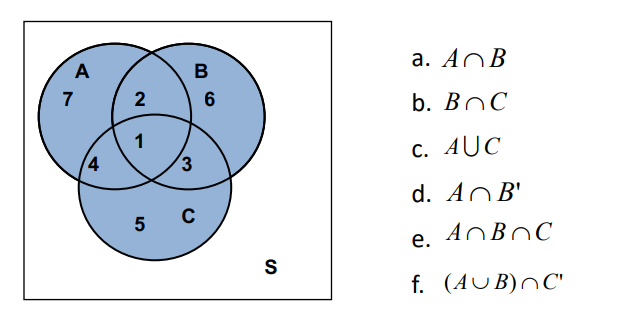
\includegraphics[]{graphics/q1.png}
}
\end{problem}

\subsection*{Answer 1}

\begin{enumerate}[a.]
	\item \( A \cap B = \{ 1, 2 \} \)
	\item \( B \cap C = \{ 1, 2, 3 \} \)
	\item \( B \cup C = \{ 1, 2, 3, 4, 5, 7 \} \)
	\item \( A \cap B' = \{ 4 \} \)
	\item \( A \cap B \cap C = \{ 1 \} \)
	\item \( ( A \cup B ) \cap C' = \{ 2, 6, 7 \} \)
\end{enumerate}

\section*{Question 2}
\begin{problem}
Do males or females feel more tense or stressed out
at work? A survey of employed adults conducted online by Harris Interactive
on behalf of the American Psychological Association revealed the following:

\begin{enumerate}[a.]
	\item Give an example of a simple event.
	\item Give an example of a joint event.
	\item What is the complement of “Felt tense or stressed out at work”?
	\item Why is “Male and felt tense or stressed out at work” a joint event?
	\item Given that the employed adult felt tense or stressed out at work, what is the probability that the employed adult was a male?
	\item Given that the employed adult is male, what is the probability that he felt tense or stressed out at work?
	\item Explain the difference in the results in (a) and (b).
	\item Is feeling tense or stressed out at work and gender independent?
\end{enumerate}
\end{problem}

\subsection*{Answer 2}

\subsubsection*{2a}

A simple event might be a `Male (chooses something)'.

\subsubsection*{2b}

A joint event might be a `Female and felt tense or stressed out at work'.

\subsubsection*{2c}

A complement of `Felt tense or stressed out at work' is `Not felt tense or out at work'

\subsubsection*{2d}

It is like that because it is two event that might happen at the same time.

\subsubsection*{2e}

The probability of an employed adult male is \(\frac{244+495}{244+495+282+480} = \frac{489}{1501}\)

\subsubsection*{2f}

The probability of an employed adult male who is stressed out at work is \(\frac{244}{244+495} = \frac{244}{739}\)

\subsubsection*{2g}

Answer \textit{2e} compares an adult male against everyone (the universe), while answer \textit{2f} compares an adult male that chose yes against only adult males.

\subsubsection*{2h}

From the data above, Male have a probability of \( \frac{244}{739} \approx 0.33017\) to be tense or stressed out while female have a probability of \(\frac{282}{762} \approx 0.3700\). It is safe to say that feeling tense or stressed out at work is gender independent with an error rate of \(\approx 0.004\).

\section*{Question 3}
\begin{problem}
If \(P(A) = 0.5\), \(P(A\cap B) = 0.1 \), and \(P(A\cup B) = 0.8\). What are the possible value of \(P(B)\) and \(P(B')\)?
\end{problem}

\subsection*{Answer 3}
Since \(P(A \cup B) = 0.8 \therefore P((A \cup B)') = \textbf{0.2}\).

Following that, since \(P(A) = 0.5\), \(P((A \cup B)') = 0.2\) and \(P(A\cap B) = 0.1\), therefore \(P(B) = 1 - P((A \cup B)') - P(A) + P(A \cap B) = 0.4\). So, \(P(B') = 1 - P(B) = \textbf{0.6}\)

\section*{Question 4}
\begin{problem}
A car repair is either on time or late and either satisfactory or unsatisfactory. If a repair is made on time, then there is a probability of 0.85 that is satisfactory. There is a probability of 0.77 that a repair will be made on time. What is the probability that a repair is made on time and is satisfactory?
\end{problem}

\subsection*{Answer 4}
Let an on time car repair to be \(T\) and a satisfactory car repair to be \(S\). Then
\[
	\begin{aligned}
		P(T \cap S)     & = 0.85                               \\
		P(T)            & = 0.77                               \\
		P(T \implies S) & = 0.77 \times 0.85 = \textbf{0.6545} \\
	\end{aligned}
\]

\section*{Question 5}
\begin{problem}
A company sells a certain type of car that is assembles in one
of four possible locations.

\medskip

\begin{itemize}
	\item Plant I supplies 20\% of the cars
	\item Plant II 24\%
	\item Plant III 25\%
	\item Plant IV 31\%
\end{itemize}

\medskip

A customer buying a car does not know where the car has been assembled. A car assembled in plant I has a probability of 0.05 of receiving a claim on its warranty, plant II is 0.11, plant III is 0.03, and plant IV is 0.08. Calculate:

\begin{enumerate}[a.]
	\item The probability that a claim on the warranty of the car will be required.
	\item If a claim is made on the warranty of the car, how does this change these probabilities in plant I, II, III, and IV\@?
\end{enumerate}
\end{problem}

\subsection*{Answer 5}

Lets agree that the probability of plant \(x\) receiving a claim on its warranty is \(P(W_x)\).

\subsubsection*{5a}

\[
	\begin{aligned}
		P(W) & = (0.2 \cdot 0.05) + (0.24 \cdot 0.11) + (0.25 \cdot 0.03) + (0.31 \cdot 0.08) \\
		P(W) & = 0.1 + 0.0264 + 0.0075 + 0.0248                                               \\
		P(W) & = \textbf{0.1587}                                                              \\
	\end{aligned}
\]

\subsubsection*{5b}

Assume that the customer does not have the knowledge of which plant their car is made from, this is just a weighted sum of all the probabilities. Given a car that's manufactured in a known plant, the probability of the said car to have a claimed warranty is straight the probability that's mentioned on the question.


% \printbibliography[]{}


\end{document}
